%====================================================================================
\section{Modelando el componente irregular}
%====================================================================================

%------------------------------------------------------------------------------------
\subsection{Modelos AR, MA y ARMA}
%------------------------------------------------------------------------------------

%---------------------------------------------------
\subsubsection{Proceso Autorregresivo (AR)}
%---------------------------------------------------

\begin{frame}{Proceso Autorregresivo $(AR)$}
	Definimos un \textcolor{red}{proceso autorregresivo de primer orden $AR(1)$} omo un proceso aleatorio que responde a una expresión del tipo
		$$Z_t = \rho_0 + \rho_1 Z_{t-1} + a_t \textup{ o bien } \breve{Z}_{1} = \rho_1\breve{Z}_{t-1}+a_t \textup{con} \breve{Z}_{t} = Z_t - \rho_0$$
	Para que el proceso $AR(1)$ sea estacionario se debe cumplir que $-1<\rho_1<1$ para que $\sigma_{Z}^2$ finita y no negativa.
		$$Var(\breve{Z}_{t}) = \sigma_{Z}^2 = \rho_1^2\sigma_{Z}^2 + \sigma_{a}^2 = \frac{\sigma_{a}^2}{1-\rho_1^2}$$
	Los procesos autoregresivos pueden generalizarse al orden $p$ \textcolor{red}{$AR(p)$}  sin más que añadir términos retardados en la expresión general.
		$$Z_t = \rho_0 + \rho_1 Z_{t-1} + \rho_2 Z_{t-2} + \ldots \rho_p Z_{t-p} + a_t$$
\end{frame}
%---------------------------------------------------
\begin{frame}{Simulación de dos procesos $AR(1)$}
	\centering
	\begin{figure}
		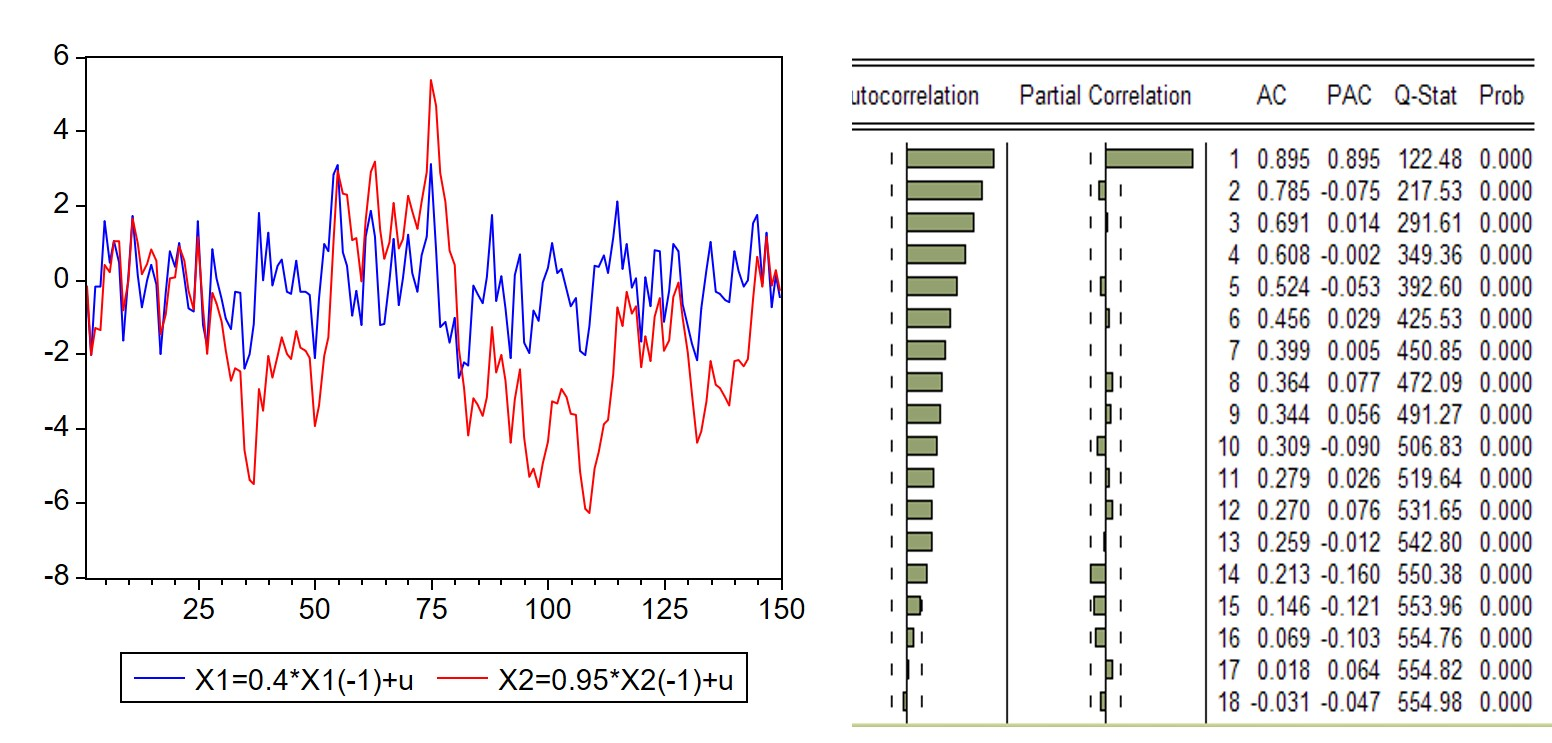
\includegraphics[width = 0.99\linewidth]{fig/figure8.jpg}
	\end{figure}
\end{frame}
%---------------------------------------------------
\begin{frame}{Función de autocorrelación (FAC) de un $AR(1)$}
	$$\widehat{\rho}_k = \frac{\gamma_k}{\gamma_0}=\phi^{k}; \textup{ donde } \phi \textup{ es el coeficiente que acompaña a } Z_{t-1}$$
	
	Por último, la función de autocorrelación parcial se corta de forma abrupta después del primer rezago.\\
	
	Es fácil ver por qué del corte. Las autocorrelaciones parciales son precisamente los últimos coeficientes en una regresión, por lo que en un proceso $AR(1)$ los coeficientes de los rezagos más largos son cero.	
\end{frame}

%---------------------------------------------------
\subsubsection{Medias móviles (MA)}
%---------------------------------------------------
\begin{frame}{Medias móviles $(MA)$}
	Definimos una \textit{media móvil} de primer orden $MA(1)$ como un proceso aleatorio que responde a una expresión del tipo
		$$Z_t = a_t + \theta_1a_{t-1}$$
	Los procesos de medias móviles son estacionarios pueden generalizarse al orden $q$ $MA(q)$ sin más que añadir términos retardados en la expresión general.
		$$Z_t = a_t + \theta_{}1a_{t-1}+\theta_{2}a_{t-2} + \ldots + \theta_{q}a_{t-q}$$
\end{frame}
%---------------------------------------------------
\begin{frame}{Simulación de dos procesos $AR(1)$}
	\centering
	\begin{figure}
		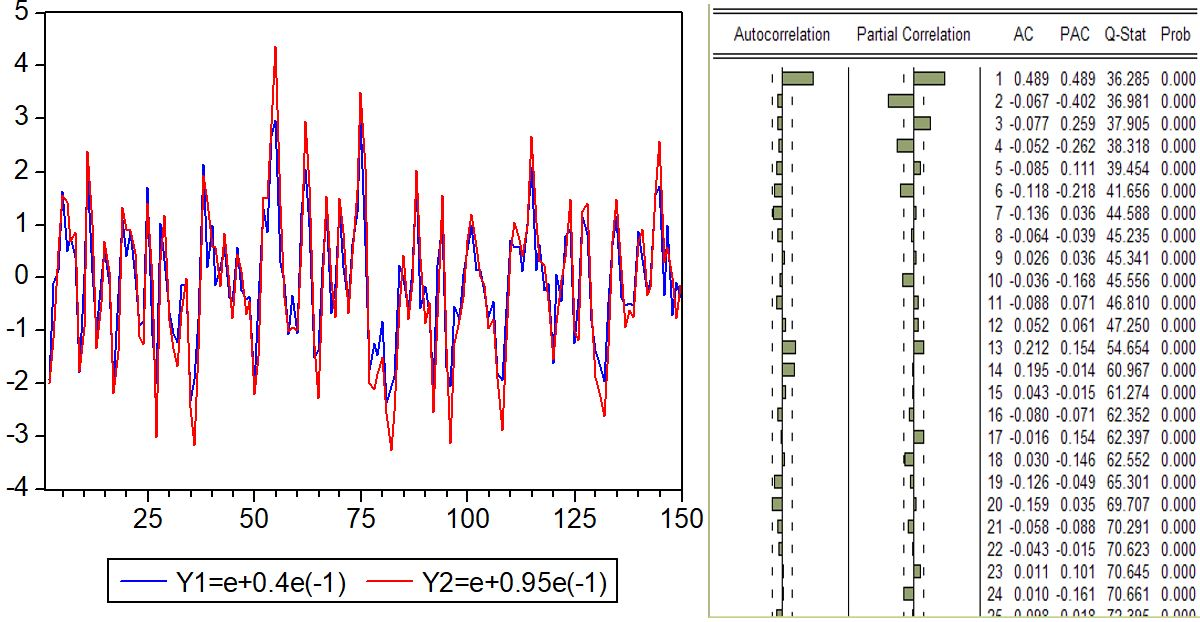
\includegraphics[width = 0.99\linewidth]{fig/figure9.jpg}
	\end{figure}
\end{frame}
%---------------------------------------------------
\begin{frame}{Función de autocorrelación (FAC) de un $MA(1)$}
	\begin{equation*}
		\widehat{\rho}_k = \frac{\gamma_k}{\gamma_0} \begin{cases}
													 	\frac{\theta}{1-\theta^2} &, k=1\\
													 	0 &, k>1
													 \end{cases}
	\end{equation*}
	Nótese que los requisitos de estacioneriedad (media y varianza constante+autocorrelación que depende del desplazamiento) se cumplen para cualquier MA independiendemente de sus parámetros.\\
	
	Si además $|\theta|<1$ se dice que el proceso $MA(1)$ es invertible en el sentido que puede ser representado por una serie que depende del pasado de la propia serie en vez del pasado de los errores
\end{frame}

%---------------------------------------------------
\subsubsection{Herramientas de identificación}
%---------------------------------------------------
\begin{frame}{Herramientas de identificación: Correlograma}
	\centering
	\begin{figure}
		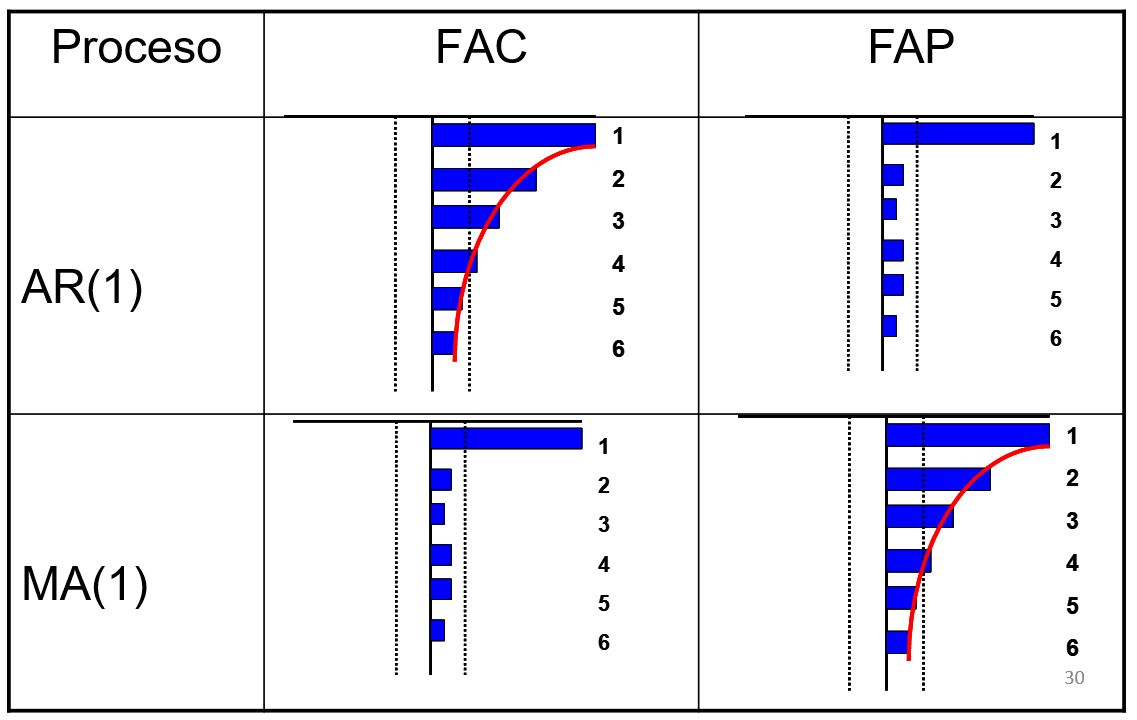
\includegraphics[width = 0.85\linewidth]{fig/figure10.jpg}
	\end{figure}
\end{frame}
%---------------------------------------------------
\begin{frame}{Herramientas de identificación: Correlograma}
	\centering
	\begin{figure}
		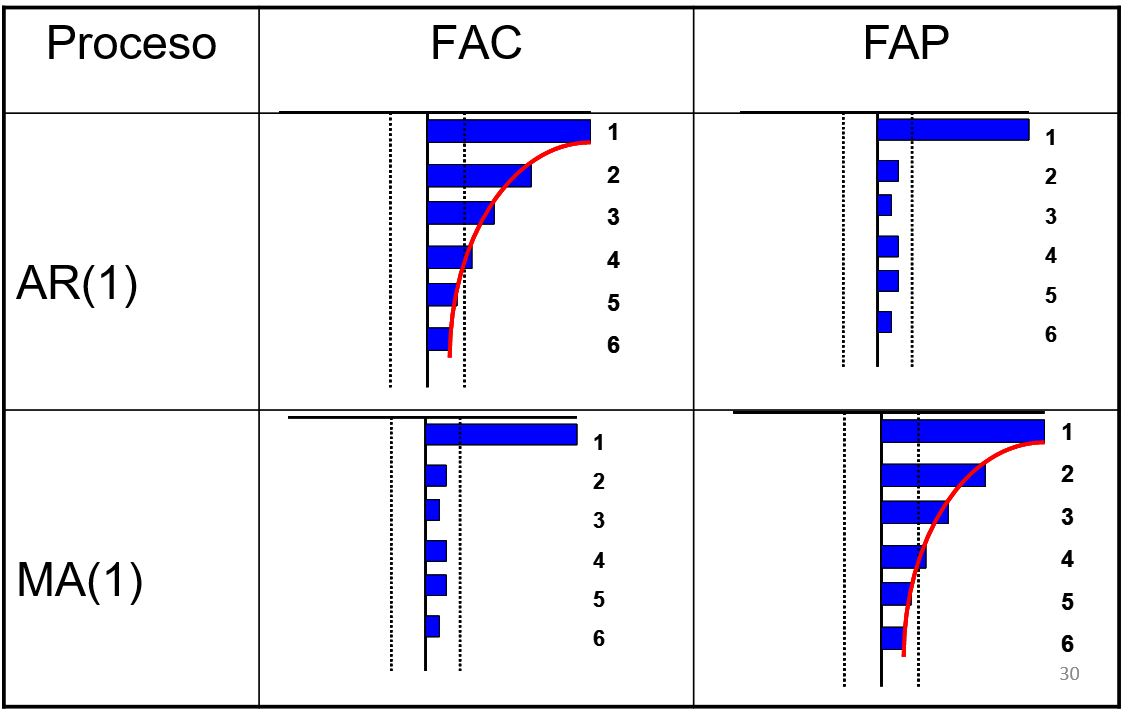
\includegraphics[width = 0.85\linewidth]{fig/figure11.jpg}
	\end{figure}
\end{frame}

%---------------------------------------------------
\subsubsection{Promedios móviles autoregresivos (ARMA)}
%---------------------------------------------------
\begin{frame}{Promedios móviles autoregresivos (ARMA)}
	Es una combinación de un proceso AR y uno MA. La representación más sencilla es la de un ARMA(1,1)
		$$Z_t = \rho_1\breve{Z}_{t-1} +a_t +\theta a_{t-1} \textup{ con }  \breve{Z}_t = Z_t - \rho_0$$
	Como antes, para que el proceso sea estacionario se debe cumplir que $-1<\rho_1<1$ y para que sea invertible $-1<\theta<1$
\end{frame}